% Title: gl2ps_renderer figure
% Creator: GL2PS 1.4.2, (C) 1999-2020 C. Geuzaine
% For: Octave
% CreationDate: Thu Jun 13 07:41:35 2024
\setlength{\unitlength}{1pt}
\begin{picture}(0,0)
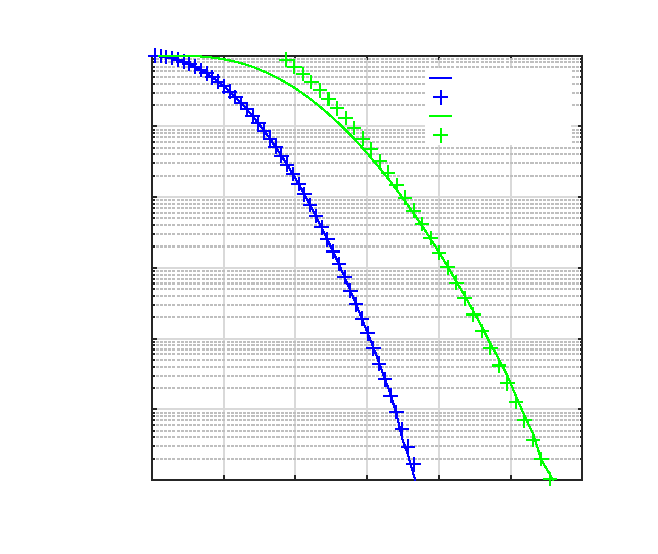
\includegraphics[scale=1]{rayleigh_sum-inc}
\end{picture}%
\begin{picture}(300,250)(0,0)
\fontsize{6}{0}\selectfont\put(39,22.8164){\makebox(0,0)[t]{\textcolor[rgb]{0.15,0.15,0.15}{{0}}}}
\fontsize{6}{0}\selectfont\put(77.75,22.8164){\makebox(0,0)[t]{\textcolor[rgb]{0.15,0.15,0.15}{{1}}}}
\fontsize{6}{0}\selectfont\put(116.5,22.8164){\makebox(0,0)[t]{\textcolor[rgb]{0.15,0.15,0.15}{{2}}}}
\fontsize{6}{0}\selectfont\put(155.25,22.8164){\makebox(0,0)[t]{\textcolor[rgb]{0.15,0.15,0.15}{{3}}}}
\fontsize{6}{0}\selectfont\put(194,22.8164){\makebox(0,0)[t]{\textcolor[rgb]{0.15,0.15,0.15}{{4}}}}
\fontsize{6}{0}\selectfont\put(232.75,22.8164){\makebox(0,0)[t]{\textcolor[rgb]{0.15,0.15,0.15}{{5}}}}
\fontsize{6}{0}\selectfont\put(271.5,22.8164){\makebox(0,0)[t]{\textcolor[rgb]{0.15,0.15,0.15}{{6}}}}
\fontsize{6}{0}\selectfont\put(35.8804,27.5){\makebox(0,0)[r]{\textcolor[rgb]{0.15,0.15,0.15}{{$10^{-6}$}}}}
\fontsize{6}{0}\selectfont\put(35.8804,61.4585){\makebox(0,0)[r]{\textcolor[rgb]{0.15,0.15,0.15}{{$10^{-5}$}}}}
\fontsize{6}{0}\selectfont\put(35.8804,95.4165){\makebox(0,0)[r]{\textcolor[rgb]{0.15,0.15,0.15}{{$10^{-4}$}}}}
\fontsize{6}{0}\selectfont\put(35.8804,129.375){\makebox(0,0)[r]{\textcolor[rgb]{0.15,0.15,0.15}{{$10^{-3}$}}}}
\fontsize{6}{0}\selectfont\put(35.8804,163.333){\makebox(0,0)[r]{\textcolor[rgb]{0.15,0.15,0.15}{{$10^{-2}$}}}}
\fontsize{6}{0}\selectfont\put(35.8804,197.292){\makebox(0,0)[r]{\textcolor[rgb]{0.15,0.15,0.15}{{$10^{-1}$}}}}
\fontsize{6}{0}\selectfont\put(35.8804,231.25){\makebox(0,0)[r]{\textcolor[rgb]{0.15,0.15,0.15}{{$10^{0}$}}}}
\fontsize{5}{0}\selectfont\put(216.505,215.755){\makebox(0,0)[l]{\textcolor[rgb]{0,0,0}{{histogram X1}}}}
\fontsize{5}{0}\selectfont\put(216.505,204.757){\makebox(0,0)[l]{\textcolor[rgb]{0,0,0}{{histogram X1+X2}}}}
\fontsize{5}{0}\selectfont\put(216.505,193.259){\makebox(0,0)[l]{\textcolor[rgb]{0,0,0}{{ X1 pdf}}}}
\fontsize{5}{0}\selectfont\put(216.505,181.26){\makebox(0,0)[l]{\textcolor[rgb]{0,0,0}{{ X1+X2 pdf}}}}
\end{picture}
